\documentclass[lettersize,journal]{IEEEtran}
\usepackage{amsmath,amsfonts}
\usepackage{algorithmic}
\usepackage{array}
\usepackage[caption=false,font=normalsize,labelfont=sf,textfont=sf]{subfig}
\usepackage{textcomp}
\usepackage{stfloats}
\usepackage{url}
\usepackage{verbatim}
\usepackage{graphicx}
\usepackage{tabularx}
\usepackage{multirow}
\hyphenation{op-tical net-works semi-conduc-tor IEEE-Xplore}
\def\BibTeX{{\rm B\kern-.05em{\sc i\kern-.025em b}\kern-.08em
    T\kern-.1667em\lower.7ex\hbox{E}\kern-.125emX}}
\usepackage{balance}
\begin{document}
\title{Information Percolation Systems for Traffic Management}
\author{António Oliveira, Luis Lucas, Marcelo Couto\\M.EIC - FEUP, Porto, Portugal}

\markboth{Modeling and Simulation project, M.EIC - FEUP}%
{}

\maketitle

\begin{abstract}
    Traffic management and road network optimization are topics that have gathered quite a lot of attention from the computer science community for the last two decades, due to the relevance of the problems presented and the applicability of the area to find solutions for these problems. One of the main challenges has been the management of congestion, related specifically to route assignment and unbalanced road networks as a consequence of the latter. The work presented in this document evaluates the use of information percolation strategies to influence the route choice of the vehicles through modelling of these strategies and their impact on the development of traffic on multiple road networks. A special focus is put into evaluating the possible influence CAVs could have on this forefront, allowing for more efficient information dissemination. A simple simulation environment is developed, using the BPR function to model the flow of traffic in the network. Three different route choice strategies based on information percolation systems are modelled, including a base case, one using the idea of modern GPS/Location services like Google Maps and another founded upon the concept of Connected Autonomous Vehicles. The results of the study show that the utilisation of 'Google Maps like' applications dramatically improves the throughput of road networks, while CAVs only present a small improvement on top of the one already given by these apps.   
\end{abstract}

\begin{IEEEkeywords}
simulation, mesa-simulator, traffic-management, autonomous vehicles, CAV
\end{IEEEkeywords}

\section{Introduction}
\label{sec:Introduction}
 
In contemporary urban landscapes, the escalating challenges associated with traffic congestion and inefficient road networks have become critical issues. As cities have continued to expand, so has the demand for effective traffic management strategies. Computer Science has had an exceptionally important role in the development of these strategies, both through the exploration of simulation as a tool for testing these strategies and with the development of algorithms and techniques with the intent of managing the problems presented directly. 

One particular problem in the field of Traffic Management is elegantly depicted by the \textit{Braess Paradox}: counterintuitively, adding a road to a road network could affect negatively its flow i.e. the vehicles' travel time \footnote{\url{https://brilliant.org/wiki/braess-paradox/}}. One possible scenario in which the aforementioned problem appears is the following the on in which the newly added road is shorter in travel time, and therefore more desirable to the drivers. Accordingly, the drivers will prefer this road to the old ones and the vehicles will all choose it, causing congestion in it. In this case, the congestion was generated by a poor strategy for the choice of road by the drivers themselves, as it did not take into consideration the other users of the road or any information other than the road network's static structure i.e. the infrastructure. 

Information percolation has the potential to help define better strategies for the choice of route of a vehicle/driver, as the problem in the scenario described arose due to the driver's lack of knowledge on the road network's state at the time of choice. The project described in this paper aims precisely to explore the influence of information percolation systems as a traffic management strategy by analyzing through simulation the influence of the introduction of such systems for route assignment. A focus will be employed on testing information percolation strategies that benefit from the existence of Connected Autonomous Vehicles, aiming to test the impact that such technology could have by coupling with information dissemination.

The relevance of the work presented resides in the fact that it has the potential to inform on possible strategies based on information percolation for attenuation of congestion in road networks, which improves the quality of life of the communities using the networks. The work should culminate in a simple simulation environment with different modelled strategies, some utilizing the notion of CAVs, some reflecting a scenario already implemented in the real world. Furthermore, it should also originate some conclusions regarding the efficiency of the strategies themselves.

The remaining paper is structured in the following manner, by order:

\begin{enumerate}
    \item Some related work will be presented and analyzed
    \item The methods and materials utilized in the project will be exposed
    \item The results of the project will be displayed and analyzed
    \item The conclusions to be drawn from the results will be given
\end{enumerate}
\section{Related Work}
\label{sec:Related-Work}

\subsection{CAVs}

Intelligent transportation systems have seen considerable investment from the scientific community in the last decade. The focus of the work published has been fairly diverse. One of the main thematics reviewed is the inclusion of Connected Autonomous Vehicles in the road networks and the impact these could have, both positive and negative. One important consequence of the inclusion of CAVs in road networks in mass is the environmental changes this could lead to, which is reviewed in \cite{kopelias2020connected}. On the same front, Zhang \cite{zhang2019impact} also analyzes the problems that arise under mixed traffic congestion, focusing on intersections and other complicated scenarios and the impact of CAVs' optimal control on the energy consumption of the vehicles. Other work reviews the impact CAVs could have on road network infrastructures and their geometric elements, outlining the natural reductions of the necessary width of lanes in highways and other equivalent roads. Another principal concern is their impact on road safety. Lanhang Ye \cite{ye2019evaluating} analyzed the impact on road safety of the inclusion of CAVs in road networks at different penetration rates in simulated environments, using the frequency of dangerous situations and collisions as a metric, having concluded that their inclusion was highly beneficial to traffic safety. 

Even so, the main hope for CAVs is for them to greatly influence the ease of traffic flow. Lanhang's work \cite{ye2019evaluating} has also led to the observation, as a byproduct of the analysis, that CAVs were also useful to the ease of the stop-and-go traffic, positively affecting traffic flow in the situations reviewed. Talebpour's \cite{talebpour2016influence} work also supports this possibility, having utilized models that appropriately represent different types of communication technology and concluded that CAVs helped improve string stability and reduce shockwave formation and propagation. This study also indicated the potential of CAVs to improve overall throughput. Ye explored modelling paradigms for CAVs in \cite{ye2018modeling}, which would be important for the development of the models in this project. Ye focuses precisely on the impact of dedicated lanes for CAVs in \cite{ye2018impact}. Some of this study's conclusions once again point towards the benefits of integrating CAVs, indicating, for instance, that it would make sense to set higher speed limits for the CAV lanes, as they are capable of travelling with increased safety. 

\subsection{Vehicle Travel Time Modelling}

To model differences in behaviour on a road network and the choice of route, there is a need to first model the traffic network and obtain travel time as a consequence of the route/road's state and congestion. The \textit{Bureau of Public Roads} (BPR) function is a simple function widely used to determine vehicle travel time as a function of the current volume of the route and its capacity, commonly referred to as a link-cost function. Its name stems from the fact that it is the function used by the \textit{Bureau of Public Roads}, now \textit{Federal Highway Administration}, from the U.S. Department of Transportation. The work of \cite{gore2023modified} presents a modern version of this function, that aims to model the stochastic nature of the problem. However, the original function will be used in this project, as the added complexity it brings did not clearly benefit the study.  

\subsection{Novelties of this work}

Many of the studies carried out in the last decade focus on mixed scenarios, as have the works cited above, where manual vehicles still occupy the road networks, meaning they do not envision a penetration rate of 100\%, such as \cite{ye2018impact}. This work differs from the ones referenced in exactly this aspect, as we explore a scenario with a 100\% penetration rate of CAVs. Moreover, many of the studies made focus on the subtle behavioural differences inside a certain road or route, or in complicated specific scenarios such as junctions and intersections. The simulation developed in this project operates at a higher level of abstraction, focusing on the impact of CAVs on route choice and its consequences on overall network throughput. Moreover, the project focuses on understanding the advantages of these techniques compared to non-CAV base cases, whereas the most common works simply study the effect of Information Percolation in CAV networks with different parameters and for different scenarios, such as \cite{talebpour2018effect} and \cite{shang2017agent}.
\section{Methods \& Materials}
\label{sec:Methods-Materials}

\subsection{Tools}

To construct our simulation environment, and due to the goal of creating a simple simulation, prioritizing understanding of the models over their precision, rather simple tools were used, which do not provide specific tools for road network and vehicle-related simulation. The Mesa \footnote{\url{https://mesa.readthedocs.io/en/latest/index.html}} Agent-based simulation Python library was used to construct the main simulation logic. Mesa focuses on being a straightforward tool that enables beginners to create agent-based simulations with a discrete time step, revolving heavily around a structure composed of agent objects that implement a step function, in which all decision-making is executed. Mesa provides some different simplistic ways for visualization and allows for direct integration for visualization of graphs built using NetworkX \footnote{\url{https://networkx.org/}}, another simple tool for graph networks management and related operations, including algorithm implementations for the most common graph-related problems, such as shortest path. Another important tool for the realization of the project was Matplotlib \footnote{\url{https://matplotlib.org/}}, a Python library that possibilities the construction of elegant graph plots, which has seamless integration with the visualization mechanisms of Mesa as well.

\subsection{Simulation Environment Definition}

\textbf{Entities:}
\begin{itemize}
    \item Vehicles
\end{itemize}

\textbf{Resources:}
\begin{itemize}
    \item Route/Road Space
\end{itemize}

\textbf{Exogenous Variables:}
\begin{itemize}
    \item \textbf{Uncontrollable:}
    \begin{itemize}
        \item \textbf{Traffic Network Configuration:} the node and edges of the graph network;
        \item \textbf{Vehicle Arrival Rate:} the amount of vehicles arriving at the network in the start node per time step;
        \item \textbf{GPS Usage Ratio:} probability of using the Intelligent GPS instead of base policy (explained further ahead)
    \end{itemize}
    \item \textbf{Controllable:}
    \begin{itemize}
        \item Information Percolation Method - Vehicle Route Decision Strategy 
    \end{itemize}
\end{itemize}

\textbf{Endogenous Variables:}
\begin{itemize}
    \item \textbf{Average Travel Efficiency at 200 (ATE200):} the ratio between the shortest time necessary for the completion of a path without traffic with the average travel time (when the 200th vehicle finishes the path) - performance metric chosen due to its capability of informing on the throughput of a network regardless of its structure and of the goal path's length;
    \item \textbf{Average Travel Time at 200:} average time taken by a vehicle to cover the (when the 200th vehicle finishes the path) - performance metric chosen for its simplicity in portraying the throughput of the network;
    \item \textbf{Max Volume to Capacity Ratio at 200:} illustrates the maximum congestion of any route in the network (when the 200th vehicle finishes the path) - performance metric chosen for its simplicity in defining the unbalance between roads;
    \item \textbf{Steps until 200:} number of simulation steps (mins) until 200 vehicles complete the path - performance metric chosen due to clearly showing the difference between models for the same network in throughput, as it is not averaged and reflects the efficiency for a fixed number of vehicles; 
\end{itemize}

\textbf{Events:}
\begin{itemize}
    \item Vehicle entering the network
    \item Vehicle leaving the network
\end{itemize}

\textbf{Performance Indicator:} ATE200 $>$ 0.4

\textbf{Decision Criteria:}
\begin{itemize}
    \item If the CAV Model presents an improvement in ATE200 of more than 0.1 compared to the Descriptive Models, then the adoption of CAVs should be taken as a serious solution for traffic congestion problems
    \item If a Model fulfils the performance indicator, its usage is deemed justified by this experiment
\end{itemize}

\subsection{Road Network Modelling}

In order to represent the road network in the simulation, it was decided that a graph representation was the most suitable. In this graph representation, the nodes would correspond to the intersections of the edges, while the edges represent the roads themselves. 

The graph is a \textbf{directed graph}. For each road network, a start node and an end node are always defined. The edges' weights correspond to the estimated cost of their traversal, varying for each operation policy. A few networks were modelled, representing slightly different levels of complexity. They ought to represent connections of highways and large roads between an origin and a destination. The main ones used in the tests are represented in Figures \ref{fig:medium-road-network} and \ref{fig:large-road-network}.

\begin{figure}
    \centering
    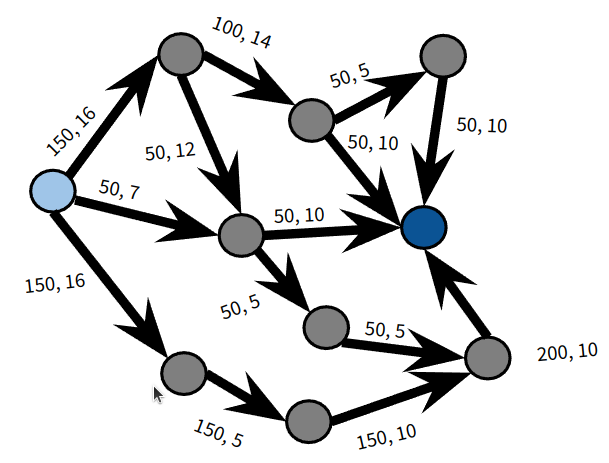
\includegraphics[width=0.4\textwidth]{img/large.png}
    \caption{Large Road Network}
    \label{fig:large-road-network}
\end{figure}

\begin{figure}
    \centering
    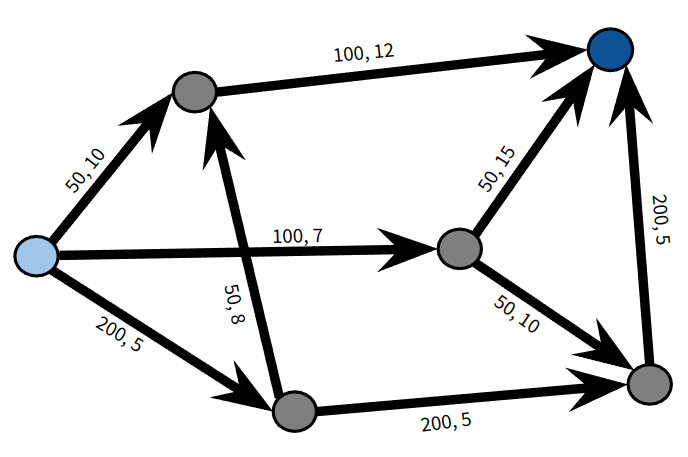
\includegraphics[width=0.4\textwidth]{img/medium.png}
    \caption{Medium Road Network}
    \label{fig:medium-road-network}
\end{figure}

\subsection{Route Choice Models}

Our simulation environment naturally defines multiple models for the representation of the road network, such as the vehicle flow model, which defines the flow of the vehicles on the network dependent on the route's characteristics and its current state regarding the vehicles that occupy it. Even so, there is only one model which is the target of this study, the route decision model: which defines the strategy followed by the agents (vehicles) for the decision between two or more different routes from their current point to their objective. This model naturally corresponds to the \textbf{operation policy} of our simulation. Taking this into account, three different models evaluated were:

\begin{itemize}
    \item \textbf{Base model:} Descriptive model based on the behaviour a vehicle would depict if the driver knew the shortest route but was oblivious to the current state of the road network in terms of volume distribution. It emulates a driver following a map or a simple GPS. Programmatically, it is emulated by having the vehicles always follow the shortest path between their current point and goal point, having this path been calculated using the free-flow time of the roads as the weights for the edges.
    \item \textbf{Intelligent GPS model:} Descriptive model attempting to represent the behaviour of a vehicle whose driver uses an application such as Google Maps, which calculates the best route taking into account the congestion of the roads in the road network, with a natural certain delay. This behaviour is coded by having the vehicles always follow the shortest path between their current point and goal point, having this path been calculated using the BPR function on the roads at a few steps prior, representing the delay in these applications.
    \item \textbf{Connected Autonomous Vehicles model:} Speculative model which describes the behaviour of the vehicles in a hypothetical scenario where they have information in real-time of the number of vehicles in each route they could opt upon and could therefore predict with very high accuracy the route with lowest travel time. This behaviour is coded by having the vehicles always follow the shortest path between their current point and goal point, having this path been calculated using the BPR function on the roads at the moment of choice, representing the instant knowledge provided by a network of autonomous vehicles, constantly in communication.
\end{itemize}

\subsection{Network Flow Modelling}

Simulating the movement of a vehicle in a road network is fundamental for the simulation task at hand. Not only that, but the travel time of the vehicle on a certain road or route should be dependent on the road's characteristics, most importantly its state at a given point in time regarding the congestion, as it is a direct function of the choices made by the drivers and impacts the network's throughput and average travel time. In order to model the movement of the vehicles and its conditioning by the state of the route at a given point in time, we chose to use the BPR (Bureau of Public Roads) function. It is a function that defines the travel time of a given vehicle through a route in function of the capacity of the route and its current volume, as well as the free-flow travel time. 

\begin{equation} \label{eq:bpr}
    T_a  = T_f \times (1 + \alpha \times (\frac{V}{C})^\beta)
\end{equation}

where:

\begin{itemize}
    \item $T_a$ is the travel time for a vehicle entering the road
    \item $T_f$ is the travel time for that road under free flow conditions (no traffic)
    \item $V$ is the current volume of the road (number of vehicles)
    \item $C$ is the capacity of the road (number of vehicles)
    \item $\alpha$ and $\beta$ are two configurable parameters. The  $\alpha$ parameter is the ratio of travel time per unit distance and $\beta$ determines how fast the curve increases from the free-flow travel time \cite{anwar2011newly}
\end{itemize}

For our experiments, we assigned the most typical values for the two constants \cite{gore2023modified}, having defined $\alpha = 0.15$ and $\beta = 4.0$.

At each time step, the agents on the simulation (the vehicles) will increment a counter denoting the progress on a given road. The vehicle will only exit the road when this counter reaches a value calculated at the point the agent made the choice to enter it. This value is exactly the value given by the BPR function, using the $C$ and $V$ values of the road in which the vehicle is entering at the moment he is entering.

\subsection{Verification}

The model was verified through extensive unit testing of the used classes with the \textit{Pytest} framework. It successfully passed all the tests it was put through, resulting in the verification of its operation inside the context of the simulation model we aimed to build and its assumptions.

\section{Results \& Discussion}
\label{sec:Results-Discussion}

\subsection{Scenarios}

The scenarios tested were a combination of the following values for the variables:

\begin{itemize}
    \item \textbf{Operation Policty:} Base, (Intelligent) GPS, CAV
    \item \textbf{Vecicle Arrival Ratio:} 15, 20, 35
    \item \textbf{Traffic Network:} Medium, Large
\end{itemize}

Only the most relevant results are presented.

\subsection{Results}

The experiments yielded fairly consistent results through the scenarios. Most results present are referent to the large network, as the differences between the models are more evident with it. A more comprehensive list of results can be found in Table \ref{tab:table}. As can be observed in Figure \ref{fig:steps-20-large}, the CAV and the Intelligent GPS policies lead to a significantly shorter time until 200 vehicles have arrived at the destination of the large network in comparison to the base case. 
CAV and Intelligent GPS models have obtained quite similar results for Average Travel Time and Average Travel Efficiency, with very similar plots and values at the 200-vehicle mark, as shown by Figures \ref{fig:ate-20-large} and \ref{fig:att-20-large}, with the CAV strategy taking the edge ever so slightly. However, the differences between these two models are made more evident by the Max. Congestion Rate plots, seen in Figure \ref{fig:congestion-20-large}. As presented, the CAV model's correspondent congestion metric slows down growth around the 2.0 value, presenting a much more horizontal plot and achieving much lower and more desirable congestion values overall, whereas the congestion on the other strategies scales near linearly. Even though congestion is not the main metric used to judge the operation policies, it is still an interesting observation. 

\begin{figure}
    \centering
    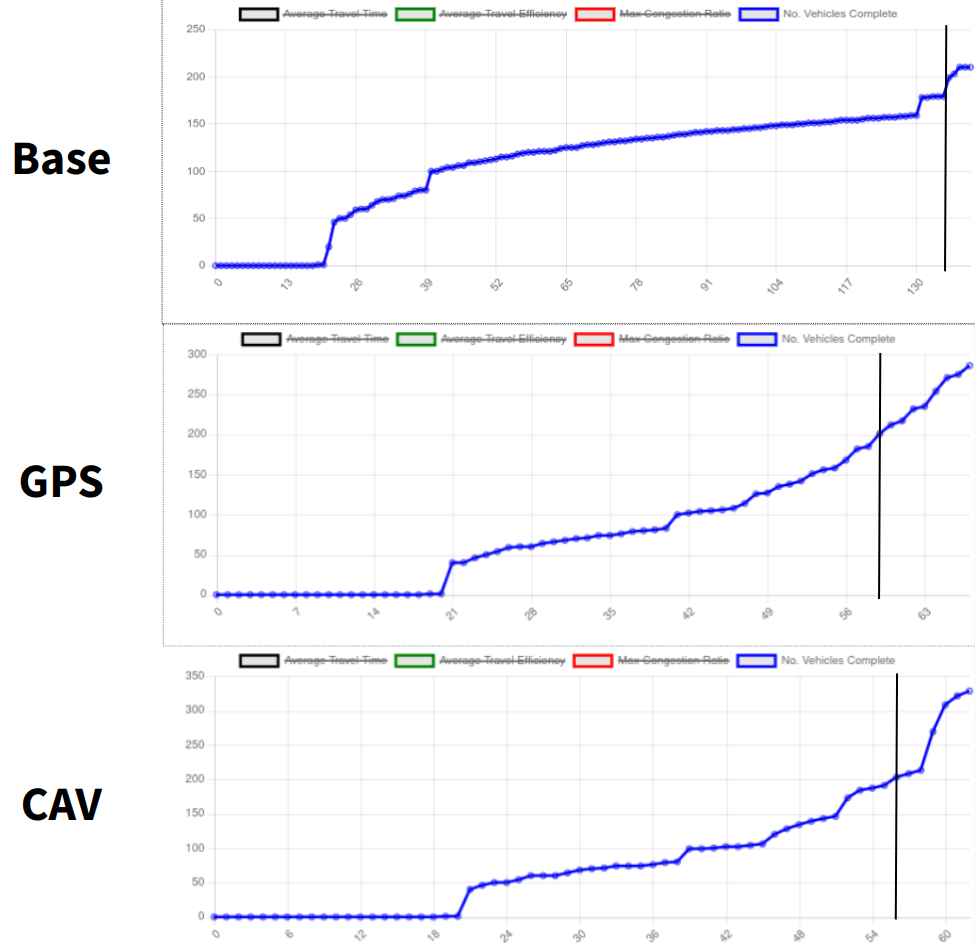
\includegraphics[width=0.45\textwidth]{img/steps-20-large.png}
    \caption{Comparison between the 3 policies on Vehicles Completed per Step for 20 vehicle Arrival Rate in the Large Network}
    \label{fig:steps-20-large}
\end{figure}

\begin{figure}
    \centering
    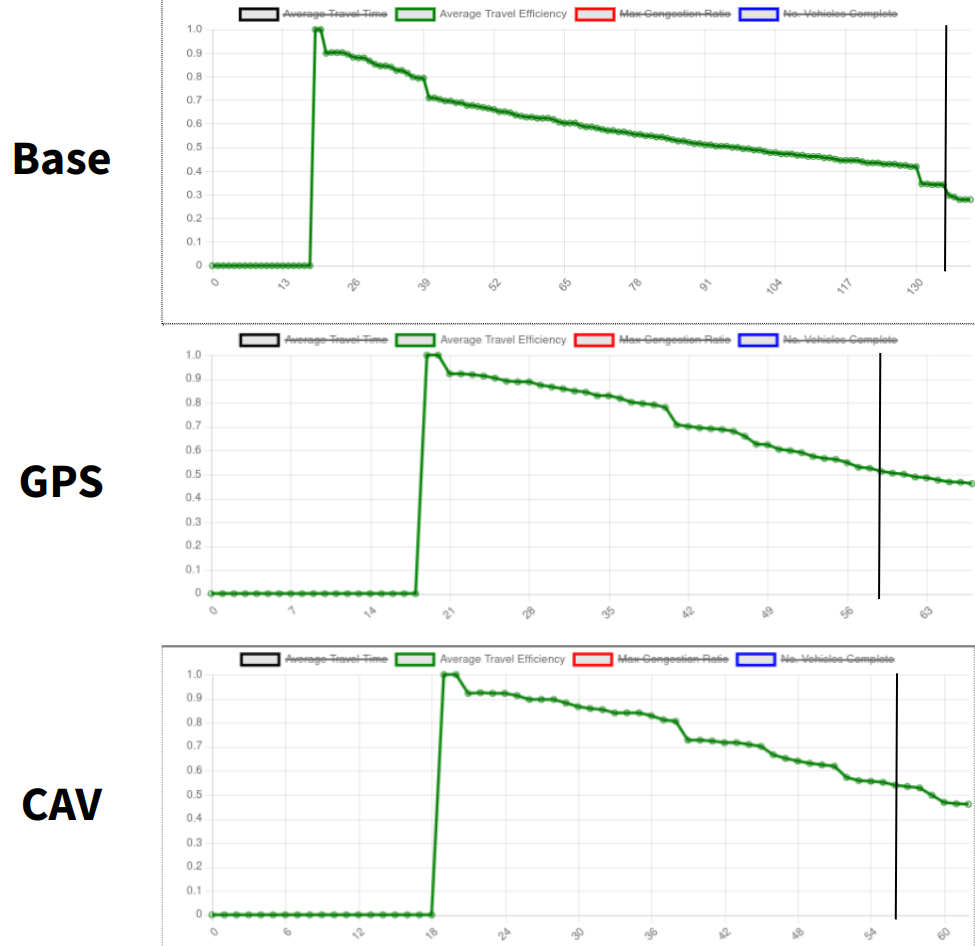
\includegraphics[width=0.45\textwidth]{img/ate-20-large.png}
    \caption{Comparison between the 3 policies on Average Travel Efficiency for 20 vehicle Arrival Rate in the Large Network}
    \label{fig:ate-20-large}
\end{figure}

\begin{figure}
    \centering
    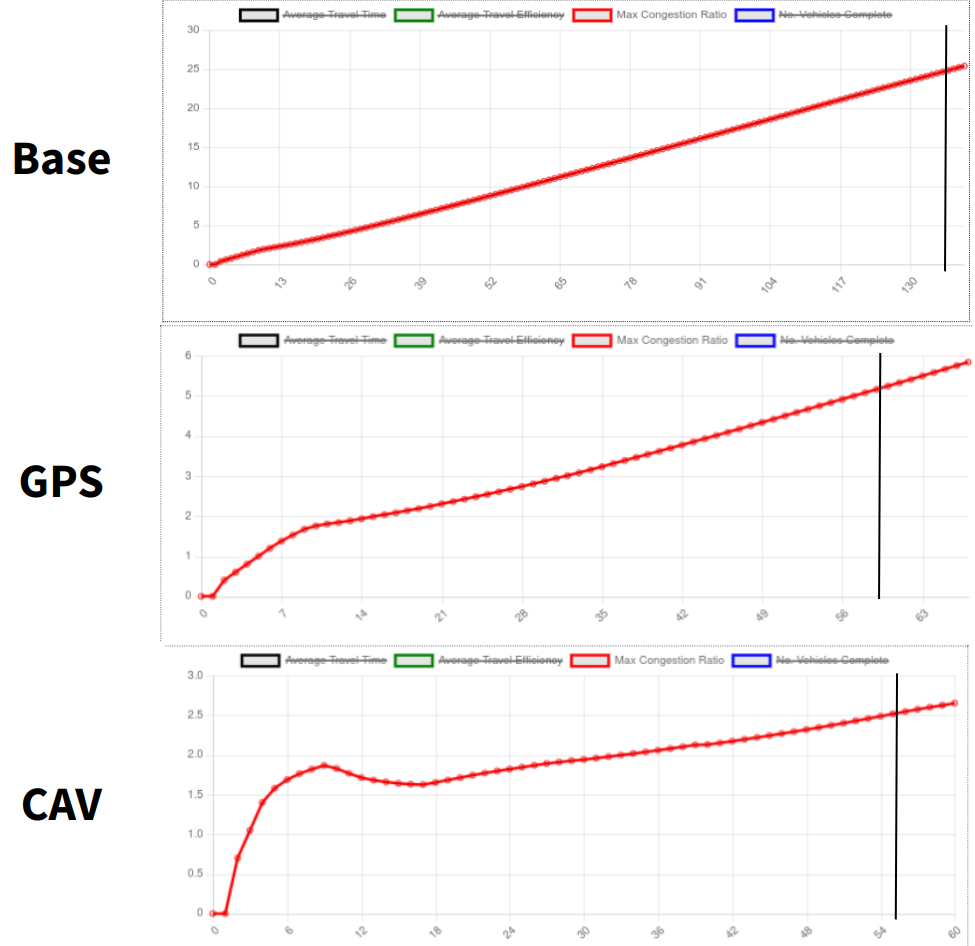
\includegraphics[width=0.45\textwidth]{img/congestion-20-large.png}
    \caption{Comparison between the 3 policies on Average Max. Congestion for 20 vehicle Arrival Rate in the Large Network}
    \label{fig:congestion-20-large}
\end{figure}

\begin{figure}
    \centering
    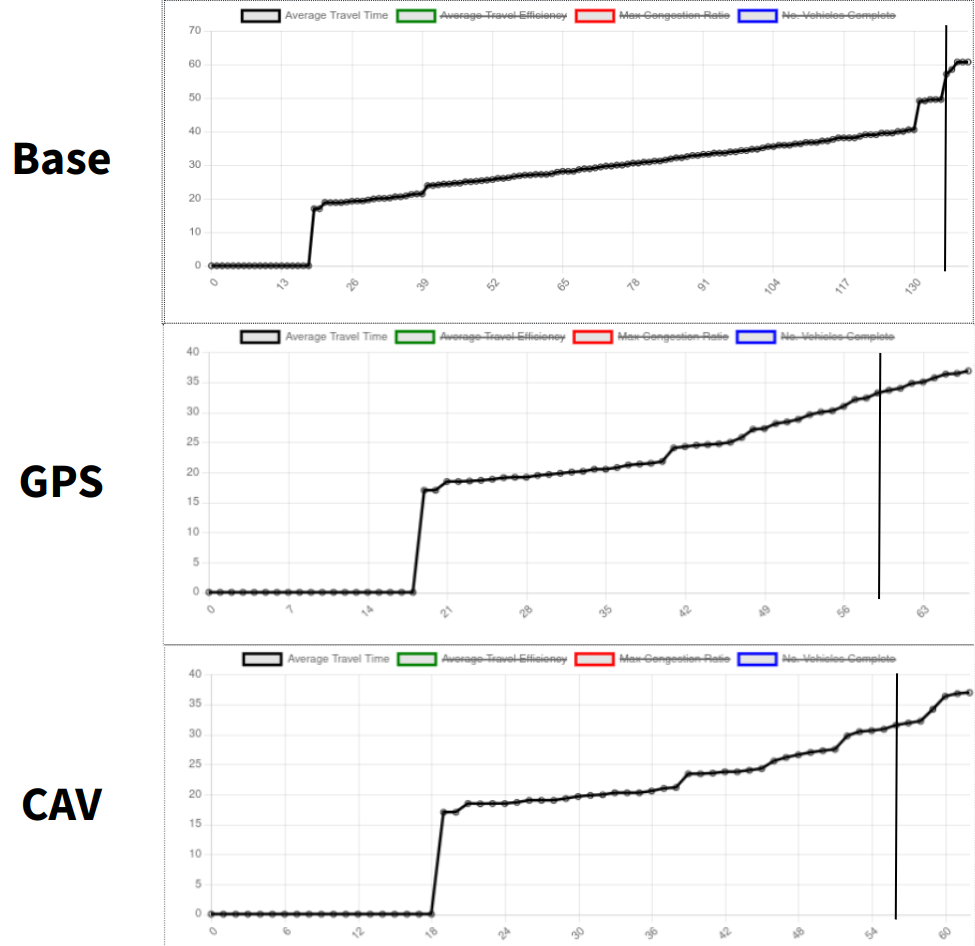
\includegraphics[width=0.45\textwidth]{img/att-20-large.png}
    \caption{Comparison between the 3 policies on Average Travel Time for 20 vehicle Arrival Rate in the Large Network}
    \label{fig:att-20-large}
\end{figure}

\begin{table*}[h]
\centering
\caption{Results by Scenario and Policy}
\begin{tabularx}{\textwidth}{|l|l|X|X|X|X|}
\hline
\textbf{Scenario} & \textbf{Policy} & \textbf{Average Travel Time (s)} & \textbf{Average Max V/C Ratio} & \textbf{Average Travel Efficiency} & \textbf{Vehicles Killed} \\ \hline
\multirow{3}{*}{Medium Model(20)}  & DUMB       & 103.80 & 26.56 & 0.193 & 1226  \\ \cline{2-6} 
                               & HALF\_SMART & 22.32  & 1.16  & 0.896 & 9538  \\ \cline{2-6} 
                               & SMART      & 26.00  & 1.47  & 0.769 & 9218  \\ \hline
\multirow{3}{*}{Large Model(15)}   & DUMB       & 104.45 & 69.86 & 0.163 & 316   \\ \cline{2-6} 
                               & HALF\_SMART & 45.32  & 33.91 & 0.375 & 3728  \\ \cline{2-6} 
                               & SMART      & 44.29  & 1.66  & 0.384 & 6774  \\ \hline
\end{tabularx}
\label{tab:table}
\end{table*}

\subsection{Discussion}

Through the analysis of the results, it can be deduced that:

\begin{itemize}
    \item The base strategy is definitely very far in terms of performance from the other ones, meaning the use of more recent and advanced GPS / path generation apps is justified;
    \item CAVs only present a slight improvement in comparison to the usage of the smart application, most likely due to the fact that the delay imposed is not very impactful in the scenarios examined;
    \item CAVs show significantly lower levels of congestion in comparison to the other options, leading to the conclusion that this strategy originates a more distributed and balanced road network.
\end{itemize}

Both CAV and Intelligent GPS policies fulfilled the performance indicator chosen, meaning both of these techniques are capable of being implemented with success in increasing a traffic network's throughput. However, only the second decision criterion is fulfilled, meaning the enhancement provided by the CAVs in comparison to the strategies already available does not justify its possible costs of implementation. 
\section{Conclusion}
\label{sec:Conclusion}

The work presented provides a simulation environment with three different route choice models developed: two descriptive models, using technology already matured at the moment of this experiment, while the third one bases itself on a hypothetical scenario, allowed by the advancements in Autonomous Driving and in the Automotive Industry. All the models developed base the traffic assignment mission on Information Percolation Strategies, which control the amount of information a vehicle has access to and therefore influence the decisions made. The project originates a simple and intuitive environment, from which more work can be built upon. The results indicate the great advantage in the usage of Intelligent Traffic/GPS applications in comparison to regular GPS or maps, as well as the little advantage CAVs could bring in this front in comparison to the aforementioned strategy. This should not, however, discourage further work in the area, as the simulation environment is quite simplistic and makes several assumptions that could hinder the results of the work but were made for the sake of the completion of the work in time.

\subsection{Future Work}

\begin{itemize}
    \item Further validation work
    \begin{itemize}
        \item improve information percolation models fidelity by validating with real-world data e.g. research Google Maps and Intelligent GPS apps further
        \item utilization of road network models that represent real scenarios  
    \end{itemize}
    \item BPR function tuning and adoption of more complex models
\end{itemize}

\section*{Acknowledgment}

This project was developed in the context of the Modelling and Simulation curricular unit, lectured by Professor Rosaldo Rossetti from the Faculty of Engineering of the University of Porto.

\appendix





\bibliographystyle{ieeetr}
\bibliography{Bib/references}

\newpage

\end{document}
